\documentclass[11pt,letter,fleqn,english,notitlepage]{article}
\usepackage{a4}
\usepackage{babel}
\usepackage{german}
\usepackage[dvips]{rotating}
\usepackage{umlaute}
\usepackage{amsmath}
\usepackage{amssymb}
\usepackage{natbib}
\usepackage[dvips]{graphics}
\usepackage{setspace}
\usepackage{geometry}
\usepackage{epsfig}
\usepackage[dvips]{color}
\usepackage{eucal}
\usepackage{fancyhdr}
\usepackage{url}
\usepackage{watermark}
%
\lhead[\fancyplain{}{\emph{A X I S E M}}] {\fancyplain{}{\emph{A X I S E M}}}
\chead[\fancyplain{}{}]                 {\fancyplain{}{}}
\rhead[\fancyplain{}{\emph{Tarje Nissen-Meyer}}]       {\fancyplain{}{\emph{Tarje Nissen-Meyer}}}
\lfoot[\fancyplain{}{}]                 {\fancyplain{}{}}
\cfoot[\fancyplain{}{\rightmark}]         {\fancyplain{}{\thepage}}
\rfoot[\fancyplain{} {}]  {\fancyplain{}{}}
%
\title{AXISEM 1.0 Manual}
\author{Tarje Nissen-Meyer}
%
\setlength{\topmargin}{-15mm}
\setlength{\textwidth}{165mm}
\setlength{\textheight}{220mm}
\hoffset=-5pt

%%%%%%%%%%%%%%  Newcommands paper3  %%%%%%%%%%%%%%%%%%%%
%
\newcommand{\eq}{\begin{equation}} \newcommand{\en}{\end{equation}}
\newcommand{\eqa}{\begin{eqnarray}} \newcommand{\ena}{\end{eqnarray}}
\newcommand{\subearth}{\raise.15ex\hbox{$\scriptstyle\oplus$}}
\newcommand{\Earth}{\raise.15ex\hbox{$\oplus$}}
\newcommand{\br}{\mbox{${\bf r}$}} \newcommand{\bs}{\mbox{${\bf s}$}}
\newcommand{\bu}{\mbox{${\bf u}$}} \newcommand{\bv}{\mbox{${\bf v}$}}
\newcommand{\bx}{\mbox{${\bf x}$}} \newcommand{\bw}{\mbox{${\bf w}$}}
\newcommand{\bC}{\mbox{${\bf C}$}} \newcommand{\bE}{\mbox{${\bf E}$}}
\newcommand{\bG}{\mbox{${\bf G}$}} \newcommand{\bI}{\mbox{${\bf I}$}}
\newcommand{\bM}{\mbox{${\bf M}$}} \newcommand{\bT}{\mbox{${\bf T}$}}
\newcommand{\bD}{\mbox{${\bf D}$}} \newcommand{\bU}{\mbox{${\bf U}$}}
\newcommand{\bK}{\mbox{${\bf K}$}} \newcommand{\bS}{\mbox{${\bf S}$}}
\newcommand{\bA}{\mbox{${\bf A}$}} \newcommand{\bQ}{\mbox{${\bf Q}$}}
\newcommand{\bF}{\mbox{${\bf F}$}} \newcommand{\bW}{\mbox{${\bf W}$}}
\newcommand{\bP}{\mbox{${\bf P}$}} \newcommand{\bB}{\mbox{${\bf B}$}}
\newcommand{\bR}{\mbox{${\bf R}$}} \newcommand{\bGamma}{\mbox{${\bf \Gamma}$}}
\newcommand{\bX}{\mbox{${\bf X}$}}
\newcommand{\rsubr}{\br_{\rm r}} \newcommand{\rsubs}{\br_{\rm s}}
\newcommand{\bzero}{\mbox{${\bf 0}$}}
\newcommand{\bdelta}{\mbox{\boldmath $\bf \delta$}}
\newcommand{\bPsi}{\mbox{\boldmath $\bf \Psi$}}
\newcommand{\bdel}{\mbox{\boldmath $\bf \nabla$}}
\newcommand{\bNcal}{\mbox{\boldmath $\bf {\mathcal N}$}}
\newcommand{\bFcal}{\mbox{\boldmath $\bf {\mathcal F}$}}
\newcommand{\bDcal}{\mbox{\boldmath $\bf {\mathcal D}$}}
\newcommand{\bsfM}{\mbox{\boldmath $\bf {\mathsf M}$}}
\newcommand{\bsfK}{\mbox{\boldmath $\bf {\mathsf K}$}}
\newcommand{\bsfU}{\mbox{\boldmath $\bf {\mathsf U}$}}
\newcommand{\bsfF}{\mbox{\boldmath $\bf {\mathsf F}$}}
\newcommand{\bsfp}{\mbox{\boldmath $\bf {\mathsf p}$}}
\newcommand{\bsfq}{\mbox{\boldmath $\bf {\mathsf q}$}}
\newcommand{\bsfu}{\mbox{\boldmath $\bf {\mathsf u}$}}
\newcommand{\bsfv}{\mbox{\boldmath $\bf {\mathsf v}$}}
\newcommand{\bsfw}{\mbox{\boldmath $\bf {\mathsf w}$}}
\newcommand{\bsff}{\mbox{\boldmath $\bf {\mathsf f}$}}
\newcommand{\bsfQ}{\mbox{\boldmath $\bf {\mathsf Q}$}}
\newcommand{\bsfW}{\mbox{\boldmath $\bf {\mathsf W}$}}
\newcommand{\bsfB}{\mbox{\boldmath $\bf {\mathsf B}$}}
\newcommand{\bsfI}{\mbox{\boldmath $\bf {\mathsf I}$}}
\newcommand{\bsfJ}{\mbox{\boldmath $\bf {\mathsf J}$}}
\newcommand{\bsfchi}{\mbox{\boldmath $\bf {\mathsf \chi}$}}
\newcommand{\bsfXi}{\mbox{\boldmath $\bf {\mathsf \Xi}$}}
\newcommand{\bsfYcal}{\mbox{\boldmath $\bf {\mathcal Y}$}}

\newcommand{\bsfzero}{\mbox{\boldmath $\bf {\mathsf 0}$}}
\newcommand{\bsfone}{\mbox{\boldmath $\bf {\mathsf 1}$}}
\newcommand{\sP}{\mbox{$\cal P$}} \newcommand{\sR}{\mbox{$\cal R$}}
\newcommand{\sS}{\mbox{$\cal S$}}
\newcommand{\bkh}{\mbox{$\hat{\mbox{${\bf k}$}}$}}
\newcommand{\blh}{\mbox{$\hat{\mbox{${\bf l}$}}$}}
\newcommand{\bnh}{\mbox{$\hat{\mbox{${\bf n}$}}$}}
\newcommand{\bph}{\mbox{$\hat{\mbox{${\bf p}$}}$}}
\newcommand{\brh}{\mbox{$\hat{\mbox{${\bf r}$}}$}}
\newcommand{\bsh}{\mbox{$\hat{\mbox{${\bf s}$}}$}}
\newcommand{\bth}{\mbox{$\hat{\mbox{${\bf t}$}}$}}
\newcommand{\bxh}{\mbox{$\hat{\mbox{${\bf x}$}}$}}
\newcommand{\byh}{\mbox{$\hat{\mbox{${\bf y}$}}$}}
\newcommand{\bzh}{\mbox{$\hat{\mbox{${\bf z}$}}$}}
\newcommand{\bthetah}{\mbox{$\hat{\mbox{\boldmath $\bf \theta$}}$}}
\newcommand{\bphih}{\mbox{$\hat{\mbox{\boldmath $\bf \phi$}}$}}
\newcommand{\bplh}{\mbox{$\hat{\mbox{\boldmath $\bf +$}}$}}
\newcommand{\bmih}{\mbox{$\hat{\mbox{\boldmath $\bf -$}}$}}
\newcommand{\ssR}{\mbox{${\sf R}$}} \newcommand{\sszero}{\mbox{${\sf
0}$}} 

\newcommand{\uto}{\mbox{${\bf u}^{\hspace{-1.6ex}\raisebox{0.5ex}{$\scriptscriptstyle\rightarrow$}}$}} 
\newcommand{\vto}{\mbox{${\bf v}^{\hspace{-1.6ex}\raisebox{0.5ex}{$\scriptscriptstyle\rightarrow$}}$}} 
\newcommand{\vtos}{\mbox{${v}^{\hspace{-1.6ex}\raisebox{0.5ex}{$\scriptscriptstyle\rightarrow$}}$}} 
\newcommand{\Eto}{\mbox{${\bf E}^{\hspace{-1.6ex}\raisebox{1.0ex}{$\scriptscriptstyle\rightarrow$}}$}} 
\newcommand{\Tto}{\mbox{${\bf T}^{\hspace{-1.6ex}\raisebox{1.0ex}{$\scriptscriptstyle\rightarrow$}}$}} 
\newcommand{\Gto}{\mbox{${\bf G}^{\hspace{-1.6ex}\raisebox{1.0ex}{$\scriptscriptstyle\rightarrow$}}$}}
\newcommand{\ruto}{\mbox{${u}^{\hspace{-1.1ex}\raisebox{0.5ex}{$\scriptscriptstyle\rightarrow$}}$}}
\newcommand{\rvto}{\mbox{${v}^{\hspace{-1.1ex}\raisebox{0.5ex}{$\scriptscriptstyle\rightarrow$}}$}}
\newcommand{\rEto}{\mbox{${E}^{\hspace{-1.3ex}\raisebox{1.0ex}{$\scriptscriptstyle\rightarrow$}}$}}
\newcommand{\rTto}{\mbox{${T}^{\hspace{-1.4ex}\raisebox{1.0ex}{$\scriptscriptstyle\rightarrow$}}$}}
\newcommand{\svto}{\mbox{${\sf v}^{\hspace{-1.2ex}\raisebox{0.5ex}{$\scriptscriptstyle\rightarrow$}}$}} 
\newcommand{\sEto}{\mbox{${\sf E}^{\hspace{-1.3ex}\raisebox{1.0ex}{$\scriptscriptstyle\rightarrow$}}$}} 
\newcommand{\bAto}{\mbox{${\bf A}^{\hspace{-1.8ex}\raisebox{1.0ex}{$\scriptscriptstyle\rightarrow$}}$}} 
\newcommand{\Ato}{\mbox{${A}^{\hspace{-1.3ex}\raisebox{1.0ex}{$\scriptscriptstyle\rightarrow$}}$}}


\newcommand{\ufrom}{\mbox{${\bf u}^{\hspace{-1.6ex}\raisebox{0.5ex}{$\scriptscriptstyle\leftarrow$}}$}} 
\newcommand{\vfrom}{\mbox{${\bf v}^{\hspace{-1.6ex}\raisebox{0.5ex}{$\scriptscriptstyle\leftarrow$}}$}} 
\newcommand{\vfroms}{\mbox{${v}^{\hspace{-1.6ex}\raisebox{0.5ex}{$\scriptscriptstyle\leftarrow$}}$}} 
\newcommand{\Efrom}{\mbox{${\bf E}^{\hspace{-1.6ex}\raisebox{1.0ex}{$\scriptscriptstyle\leftarrow$}}$}} 
\newcommand{\Tfrom}{\mbox{${\bf T}^{\hspace{-1.6ex}\raisebox{1.0ex}{$\scriptscriptstyle\leftarrow$}}$}}
\newcommand{\rufrom}{\mbox{${u}^{\hspace{-1.1ex}\raisebox{0.5ex}{$\scriptscriptstyle\leftarrow$}}$}}
\newcommand{\rvfrom}{\mbox{${v}^{\hspace{-1.1ex}\raisebox{0.5ex}{$\scriptscriptstyle\leftarrow$}}$}}
\newcommand{\rEfrom}{\mbox{${E}^{\hspace{-1.3ex}\raisebox{1.0ex}{$\scriptscriptstyle\leftarrow$}}$}}
\newcommand{\rTfrom}{\mbox{${T}^{\hspace{-1.4ex}\raisebox{1.0ex}{$\scriptscriptstyle\leftarrow$}}$}} 
\newcommand{\svfrom}{\mbox{${\sf v}^{\hspace{-1.2ex}\raisebox{0.5ex}{$\scriptscriptstyle\leftarrow$}}$}} 
\newcommand{\sEfrom}{\mbox{${\sf E}^{\hspace{-1.3ex}\raisebox{1.0ex}{$\scriptscriptstyle\leftarrow$}}$}} 
\newcommand{\bAfrom}{\mbox{${\bf A}^{\hspace{-1.8ex}\raisebox{1.0ex}{$\scriptscriptstyle\leftarrow$}}$}}
\newcommand{\Afrom}{\mbox{${A}^{\hspace{-1.3ex}\raisebox{1.0ex}{$\scriptscriptstyle\leftarrow$}}$}} 

\newcommand{\bAboth}{\mbox{${\bf A}^{\hspace{-1.7ex}\raisebox{1.0ex}{$\scriptscriptstyle\leftrightarrow$}}$}}
\newcommand{\Aboth}{\mbox{${A}^{\hspace{-1.1ex}\raisebox{1.0ex}{$\scriptscriptstyle\leftrightarrow$}}$}}
%

%
\begin{document}
%
\pagestyle{fancy}
\thispagestyle{empty}
%

\section{PyAxi: Python interface for AXISEM}

\subsection{Introduction}
PyAxi is a Python script developed as an interface for AXISEM. 
All the options available in AXISEM are included in only one input file (\textit{inpython.cfg}).
By running the script, all the necessary steps (MESHER, SOLVER and Post-Processing) will be done automatically.
Python is the only requirement; However, some special functionalities (mseed format, plotting in Python environment) need \textit{ObsPy} to be installed. \\

\noindent \textit{Basic requirement}: Python.\\
\textit{Convert to MSEED (not obligatory)}: ObsPy (https://github.com/obspy/obspy/wiki).\\

\subsection{How to Run PyAxi?}
%In this part, we show how to run PyAxi for different input files.
First, let's check whether AXISEM can be run properly on our machine. 
For this reason:\\

Start from within the {\tt AXISEM} directory:
\begin{enumerate}
\itemsep0em
\item {\tt cd TESTING}
\item {\tt python PyAxi.py --check}
\end{enumerate}
\noindent This gives an overview of the installation status of all relevant compilers and tools required
to run AXISEM on your machine (Figure~\ref{check_pyaxi}). 
Please note that \textit{--check} does not check for all the possible compilers.
It just checks for those listed in Figure~\ref{check_pyaxi}; 
therefore, for other compilers, it should be done manually.\\

\begin{figure*}[htb]
\begin{center}
\includegraphics[scale=0.32]{check_pyaxi.eps}
%\caption{\textit{}}
\end{center}
\caption{\textit{Checking all the relevant compilers and tools required to run AXISEM.}}
\label{check_pyaxi}
\end{figure*}


\noindent After installation of all required packages, 
maybe the best way to get familiar with AXISEM is to run the code with the default input file:\\

Start from within the {\tt AXISEM} directory:
\begin{enumerate}
\itemsep0em
\item {\tt cd TESTING}
\item {\tt python PyAxi.py inpython.cfg}
\end{enumerate}

All the rest will be done automatically...\\

\noindent \textit{inpython.cfg} is a configuration file that contains all the AXISEM options.
To change the input file, open \textit{inpython.cfg} with an editor:\\

Start from within the {\tt AXISEM} directory:
\begin{enumerate}
\itemsep0em
\item {\tt cd TESTING}
\item {\tt (editor) inpython.cfg}
\end{enumerate}


%%%and it has been divided into several parts:
%%%\subsubsection{general}
%%%This section in \textit{inpython.cfg} is dedicated to how and where you want to run the code.
%%%\begin{itemize}
%%% \item \textbf{address} is the directory where you have the AXISEM code.
%%% \item \textbf{mesh\_name} is the name of the directory in which the info of the generated mesh will be stored.
%%% \item \textbf{solver\_name} is the name of the directory in which the final solution will be stored.
%%% \item \textbf{verbose} produces verbose output on the screen (recommended for debugging).
%%% \item \textbf{new\_mesh} has three possibilities.
%%%'Y' runs all steps of AXISEM from generating the mesh up to saving the waveforms.
%%%'N' uses the available mesh and continues the code.
%%%'M' gives this possibility to the user to manually change the options listed at the end of the \textbf{general} section.
%%% \item \textbf{post\_processing} perferms the post processing step automatically.
%%%\end{itemize}
%%%
%%%\noindent Please note that these options make it possible for the user to change the work-flow as it is required.
%%%For instance, if you already have done one simulation and you want to use the same mesh for another simulation,
%%%it is enough to set $new\_mesh = N$.
%%%
%%%\subsubsection{mpi\_netCDF}
%%%mpi\_netCDF options control the make flags and netCDF functionality.
%%%\begin{itemize}
%%% \item \textbf{make\_flag} adds required flag(s) for running the \textit{makemake.pl} in both MESHER and SOLVER.
%%% \item \textbf{mpi\_compiler} could be set based on your local machine. 
%%% \item \textbf{netCDF} generates one netCDF file instead of having binary output.
%%% \item \textbf{netCDF\_LIBS} and \textbf{netCDF\_INCLUDE} should be changed according to your netCDF installation.
%%%\end{itemize}
%%%\subsubsection{mesher}
%%%Major options that control the MESHER part of AXISEM have been included in this part.
%%%For more information about \textbf{model}, \textbf{period} and \textbf{no\_proc} please refer to Mesher input section.
%%%
%%%\subsubsection{solver}
%%%In this part, first we have three options \textbf{no\_simu}, \textbf{seis\_length} and \textbf{time\_step}
%%%that are identical to \textbf{number of simulations}, \textbf{seismogram length} and 
%%%\textbf{time step} defined in Solver input. Moreover:
%%%\begin{itemize}
%%% \item \textbf{source\_type} could be selected from 'sourceparams' and 'cmtsolut'.
%%% \item \textbf{receiver\_type} has three 'colatlan', 'stations' and 'database' options.
%%% \item \textbf{save\_XDMF} saves XDMF files (high resolution 2D wavefields), more options in \textit{inparam\_xdmf}.
%%% \item \textbf{force\_aniso} for anisotropic model handling.
%%%\end{itemize}
%%%\noindent Based on what we have selected in 'source\_type', one of the two parts for the source parameters
%%%should be modified, e.g. if you have chosed 'cmtsolut', then go to the \textit{cmtsolut} parameters and 
%%%change the options accordingly.
%%%\subsubsection{post\_processing}
%%%This section controls the required options for Post processing. All the parameters are identical to what has been explained in \textit{Post processing} section.
%%%\subsubsection{MISC}
%%%MISC contains the input parameters for converting the waveforms to MSEED format and convolve them with Source Time Function.
%%%These parameters are optional and need \textit{ObsPy} to be installed.
%%%\begin{itemize}
%%% \item \textbf{mseed} to convert all the seismograms to MSEED format (one file for each).
%%%These files will be located in the SEISMOGRAMS/MSEED folder in each solution directory (\textit{solver\_name}).
%%% \item \textbf{mseed\_all} to convert all the seismograms into MSEED format (one file for all).
%%%It will generate one 'seismograms.mseed' file saved in SEISMOGRAMS folder. 
%%% \item \textbf{convSTF} convolves the converted seismograms with Source Time Function (STF).
%%% \item \textbf{halfduration} determines the halfduration of the STF.
%%% \item \textbf{filter} applies a lowpass and a highpass filter with the minimum and maximum
%%%frequencies defined in \textbf{fmin} and \textbf{fmax}.
%%%\end{itemize}
%%%\subsubsection{test}
%%%This part of the input file is just for the TESTING functionality that we have in AXISEM.
%%%In normal runs, one should keep the \textit{'test'} flag to 'N' to avoid any problem.
%%%TESTING will be discussed in a seperated section.




\newpage
\section{TESTING}

This section is mainly useful for the develpers or those want to change/add/remove some parts of the code and compare the new changes with the reference solutions.
For the reference solutions, 5 different tests have been designed and 
the results from \textit{yspec} [Al-Attar \& Woodhouse (2008)] and AXISEM have been included in the \textit{TESTING/automatic} directory.
The whole procedure (running the code, compare the results and plot) is automatic with the least user intervention: \\

Start from within the {\tt AXISEM} directory:
 \begin{enumerate}
 \itemsep0em
 \item {\tt cd TESTING}
 \item {\tt python test\_axisem.py}
 \end{enumerate}

Enter test number(s) and this is all you should do! \\

\noindent As an example, we want to run the \textit{test\_axisem.py} for test number 5. (Figure~\ref{test_axisem})

\begin{figure*}[htb]
\begin{center}
\includegraphics[scale=0.4]{test_axisem.eps}
\caption{\textit{Screenshot while running test\_axisem.py}}
%\caption{\textit{}}
\end{center}
\label{test_axisem}
\end{figure*}

\noindent At the end, it plots three figures (one for each channel) 
in which the new AXISEM waveforms are compared with both the original ones and \textit{yspec} results for the same simulation.
%In Figure~\ref{channel_Z}, only the Z channel has been plotted.
It should be noted that these tests are designed for rough comparison purposes (in terms of the pulse shape and sign) and they should not be considered as a detailed benchmark with respect to YSPEC. \\

\begin{figure*}[htb]
\begin{center}
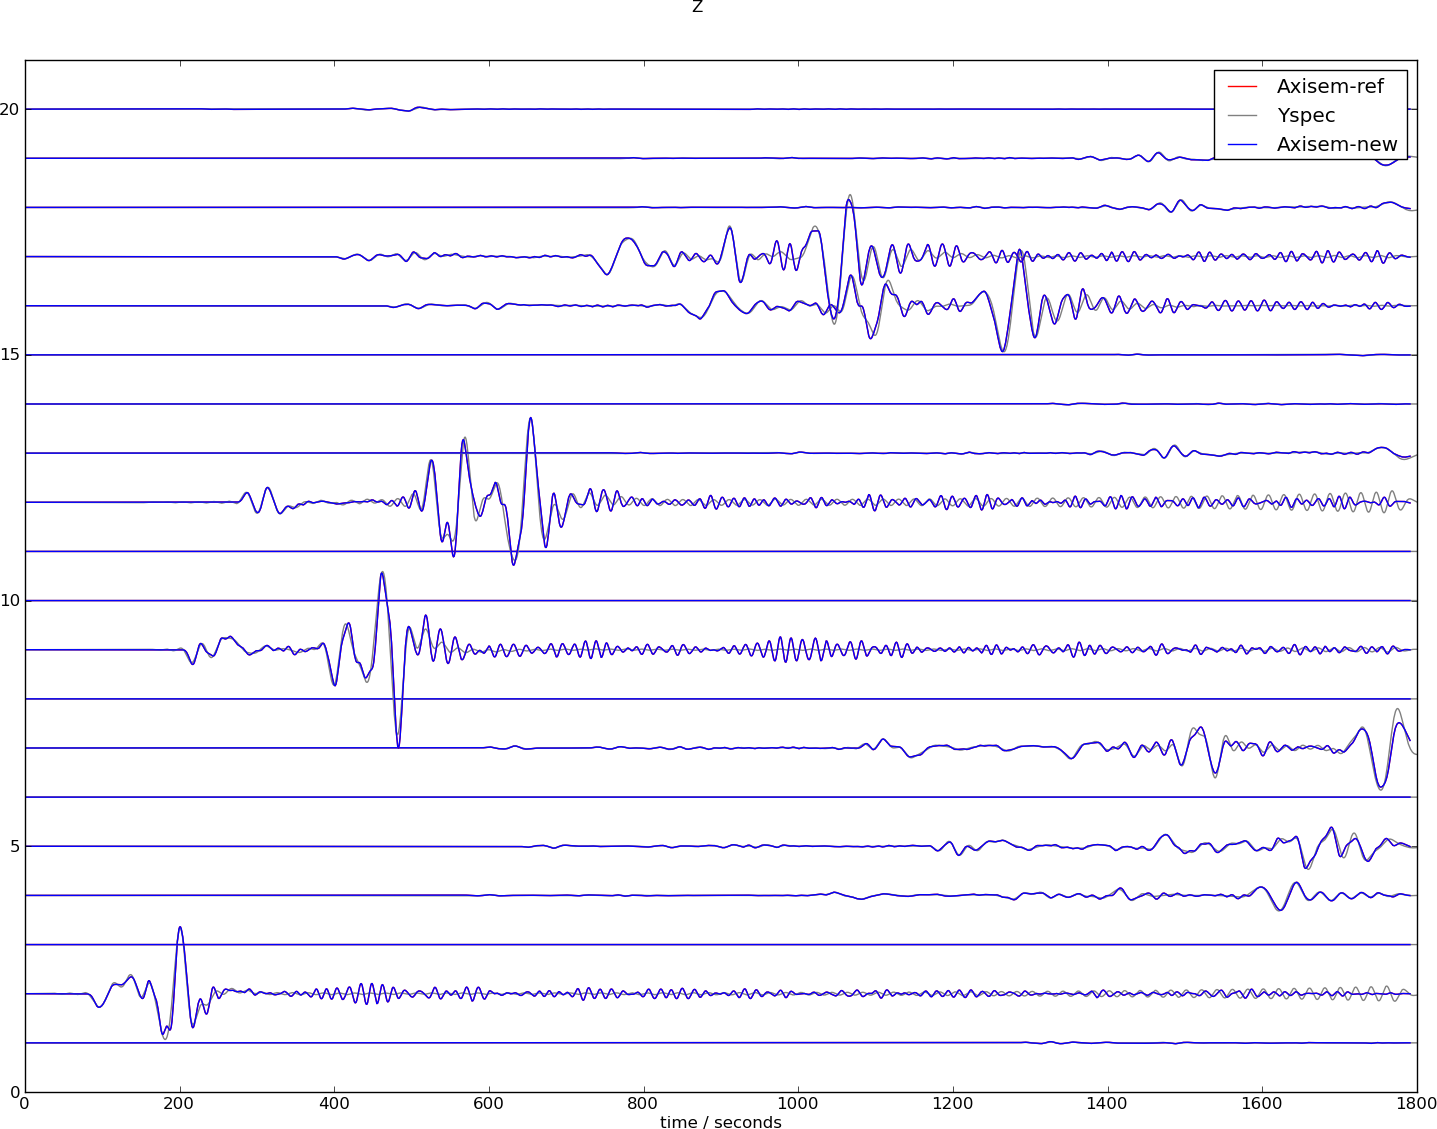
\includegraphics[scale=0.3]{record_section_Z.eps}
\caption{\textit{Comparing new AXISEM results with the reference solution and \textit{yspec} waveforms. (Z channel)}}
\end{center}
\label{channel_Z}
\end{figure*}

\noindent Another output is the \textit{l2} misfit (Figure~\ref{l2_misfit}) between the new and reference data 
in which the traces can be compared in a quantitative sense.

\begin{figure*}[htb]
\begin{center}
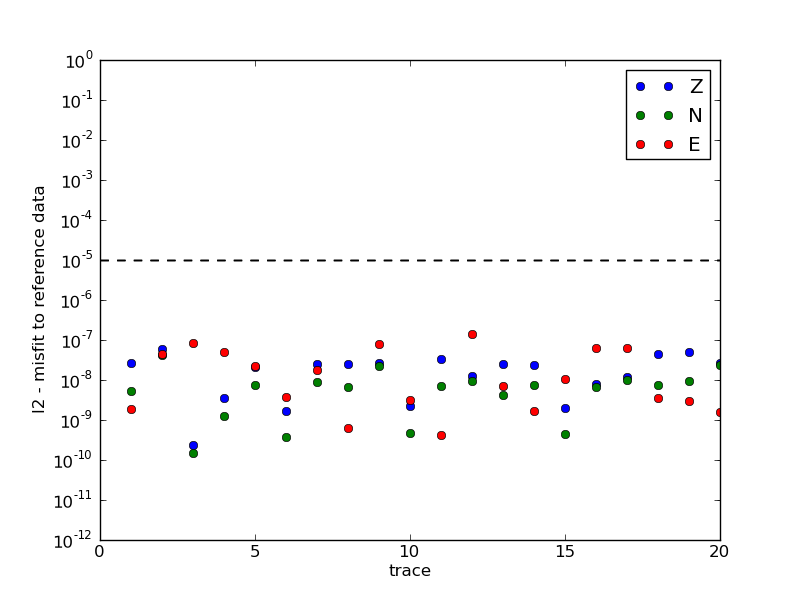
\includegraphics[width=0.8\textwidth]{l2_misfit.eps}
\caption{\textit{l2 misfit between the new and reference data.}}
\end{center}
\label{l2_misfit}
\end{figure*}

\end{document}
